\documentclass{article}   

\usepackage{geometry}
\usepackage{qtree}
\usepackage[square,numbers]{natbib}
% \usepackage{cite}  
\geometry{a4paper}

\usepackage[]{algorithm2e}
\usepackage{amsthm}
\newtheorem{theorem}{Theorem}[section]
\newtheorem{corollary}{Corollary}[theorem]
\newtheorem{lemma}[theorem]{Lemma}
\usepackage{rotating}
\usepackage[utf8]{inputenc}
\usepackage[T1]{fontenc}    % use 8-bit T1 fonts
\usepackage{lmodern}
\usepackage{hyperref}       % hyperlinks
\usepackage{lipsum}

%\usepackage[dvipsnames]{xcolor}
\usepackage{color, colortbl}

\definecolor{Gray}{gray}{0.9}
\definecolor{goldenpoppy}{rgb}{0.99, 0.76, 0.0}
\definecolor{goldenrod}{rgb}{0.85, 0.65, 0.13}

\usepackage[protrusion=true,expansion=true]{microtype}

\usepackage{amssymb}
\usepackage{amsfonts}
\usepackage{booktabs}
\usepackage{eqnarray,amsmath}
\usepackage[table]{xcolor}

\usepackage{listings}
\usepackage{dirtytalk}

\usepackage{rotating}
\usepackage{caption}

%% if you use PostScript figures in your article
%% use the graphics package for simple commands
\usepackage{graphics}


%% or use the graphicx package for more complicated commands
\usepackage{graphicx}


\usepackage{indentfirst}
\usepackage[utf8]{inputenc}
 \usepackage{subcaption}

 
\usepackage{xspace,color}
\usepackage{url}

\usepackage[export]{adjustbox}

\lstset{commentstyle=\color{red},keywordstyle=\color{black},
showstringspaces=false}
\lstnewenvironment{rc}[1][]{\lstset{language=R}}{}
\newcommand{\ri}[1]{\lstinline{#1}}  %% Short for 'R inline'

\lstset{language=R}             % Set R to default language


%https://tex.stackexchange.com/questions/96825/nicely-formatted-where-statement-for-maths
 \newenvironment{where}{\noindent{}where\begin{itemize}}{\end{itemize}}
 \renewcommand*\descriptionlabel[1]{\hspace\leftmargin$#1$}
 
\lstset{escapeinside={<@}{@>}}
% please place your own definitions here and don't use \def but
% \newcommand{}{}
%
% Insert the name of "your journal" with
% \journalname{myjournal}
%
\begin{document}

\title{%
  Practice 11: Convolutions, Chi square and covariance. } %\\~\\
  %\Large }
\author{Mayra Cristina Berrones Reyes 6291}

\maketitle

\section{Introduction}

In this work we are going to discuss in three sections the subjects of convolution, chi squared and covariance with different examples. But first, we want to give a brief introduction into these three items.

\subsection{Convolutions}

Convolution refers to a mathematical operation on two functions (\textit{f} and \textit{g}) that produce a third function (\textit{f} $*$ \textit{g}) that expresses how the shape of one is modified by the other. The term is often used both as the result function we mentioned, as well as the process of computing the function itself.\\

Convolutions can be find in several applications such as probability, statistics, computer vision, natural language processing, image and signal processing, engineering, etc.\\

The common engineering notational convention for this formula is shown in Equation \ref{eq1}, 
 \begin{eqnarray}
\label{eq1}
(f*g)(t) = \int_{-\infty}^\infty f(\tau)g(t- \tau) d\tau 
\end{eqnarray}

\begin{flushright}
$\blacksquare$
\end{flushright}


\subsection{Chi square test}

The Pearson chi squared test is a statistical test applied to show the relationship between two categorical variables. This statistic is a single number that tells how much difference exists between the observed counts and the the expected counts if there was no relationship at all in the population.\\

There are two types of chi squared tests:

\begin{itemize}
\item A chi squared goodness fit test, that determines if a sample data matches a population.
\item A chi squared test to test for independence, comparing two variables in a contingency table to see if they are related, testing whether distributions differ from each other.
\end{itemize}

The formula for the chi squared statistic test used in this type of tests is shown in Equation \ref{eq2}, 
 \begin{eqnarray}
\label{eq2}
x_{c}^2 = \sum \frac{(O_i - E_i)^2}{E_i}
\end{eqnarray}

\begin{flushright}
$\blacksquare$
\end{flushright}

\subsection{Covariance}

In mathematics and statistics, covariance is a measure of the relationship that two random variables have with each other. It evaluates how much the variables change together, but they do not measure the dependency between variables. The variance can take any positive or negative value. This values can be interpreted as:

\begin{itemize}
\item \textbf{Positive:} Indicates that two variables tend to move in the same direction.
\item \textbf{Negative:} Reveals that two variables tend to move in an inverse direction.
\end{itemize}

The formula for the covariance between two random variables $X$ and $Y$ can be calculated using  Equation \ref{eq3}, 
 \begin{eqnarray}
\label{eq3}
Cov(X,Y) =  \frac{\sum(X_i - \overline{X})(Y_j - \overline{Y})}{n}
\end{eqnarray}

\begin{flushright}
$\blacksquare$
\end{flushright}


\section{Section 1: Convolutions}
\textit{Identify an application of your interest from the subject of convolution and present some related contribution (theoretical or numerical) }\\

Convolutions, as we see in the introduction of this work, are an extremely general idea. The expression used in Equation \ref{eq1} can also be used in a higher number of dimensions. Just like with one dimensional convolutions, the concept of two dimensional convolutions can be imagined as sliding one function on top of another, multiplying and adding \cite{twds}. \\

Our subject of interest, and one of the common application of convolutions is image processing. In this case, we think of the images as two dimensional functions, in the form of value of pixels. Many important image transformations such as noise additions, sharpening of the image, etc. are convolutions where we convolve the image function with a very small local function called \say{kernel}. The kernel slides to every position of the image and computes a new pixel as a weighted sum of pixels as it floats over.\\

\begin{table}[]\caption{Some popularly known kernels for image processing.}\label{tab1}
\centering
\begin{tabular}{ c c c c }
\toprule
\textbf{Boxblur} & \textbf{Gaussian blur} &\textbf{Identity} & \textbf{Sharpen} \\
\midrule\\
\addlinespace[-2ex]
$ \frac{1}{9}\begin{bmatrix}  1 & 1 & 1\\ 1 &  1 & 1 \\ 1 & 1 & 1\end{bmatrix}$ &
$\frac{1}{16} \begin{bmatrix} 1 & 2 & 1 \\ 2 & 4 & 2 \\ 1 & 2 & 1 \end{bmatrix}$&
$ \begin{bmatrix} 0 & 0 & 0 \\ 0 & 1 & 0 \\ 0 & 0 & 0 \end{bmatrix}$&
$ \begin{bmatrix} 0 & -1 & 0 \\ -1 & 5 & -1 \\ 0 & -1 & 0 \end{bmatrix}$\\
\bottomrule
\end{tabular}
\end{table}

In Table \ref{tab1} we see some examples of popularly kernels used for different types of image precessing. Depending on the scale it wants to work, we can change the size of its matrix and some of the numbers inside the matrix. \\

The easiest way of representing how exactly a kernel works, can be appreciated in Figure \ref{fig1} where we can see the kernel sweeping over the image matrix. We multiply a batch of the image with the kernel, and then calculate the cumulative sum to add it to another matrix.\\

\begin{figure}[]
  \centering
  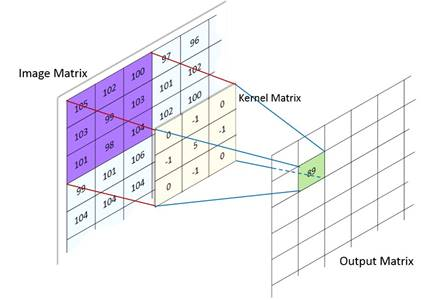
\includegraphics[width=.8\linewidth]{kernel2.jpg}  
	\caption{Graphical example of how a kernel works in a convolution of an image \cite{stda}.}
\label{fig1}
\end{figure}

As an example of the use of convolutions in image processing, we can use the library of \texttt{magick} \cite{magik} in \texttt{R} that already has some integrated values for the kernels to add noise, edge detection, sharpen image, etc. In Figure \ref{fig2} we see some of this examples. In this figure we also add a hand made kernel to blur the image, based on the values we used in Table \ref{tab1}. \\

\begin{figure}[]
\begin{subfigure}{.3\textwidth}
  \centering
  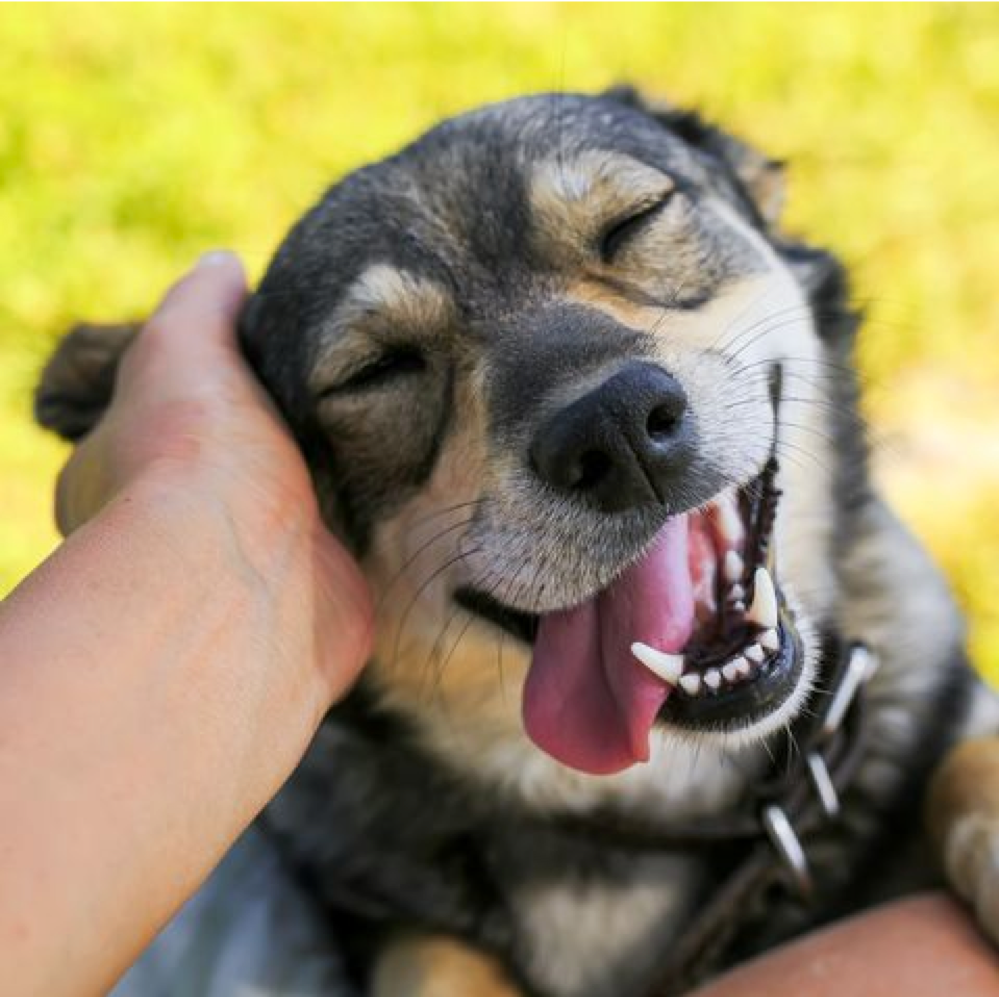
\includegraphics[width=.9\linewidth, left]{pup_original.png}  
  \caption{Original image}
  \label{sb2-1}
\end{subfigure}\hspace{5mm}%
\begin{subfigure}{.3\textwidth}
  \centering
  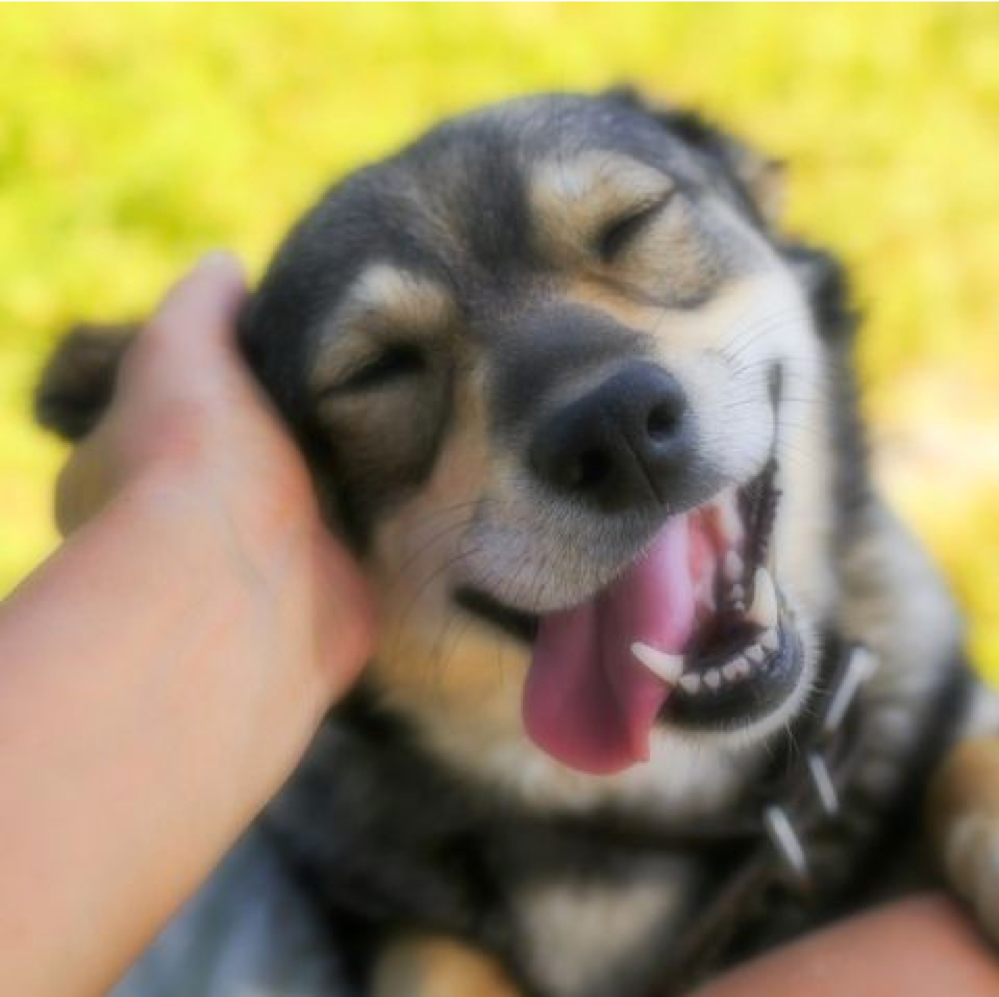
\includegraphics[width=.9\linewidth]{pup_gaus.png}  
  \caption{Convolution with the gaussian kernel}
  \label{sb2-2}
\end{subfigure}\hspace{5mm}%
\begin{subfigure}{.3\textwidth}
  \centering
  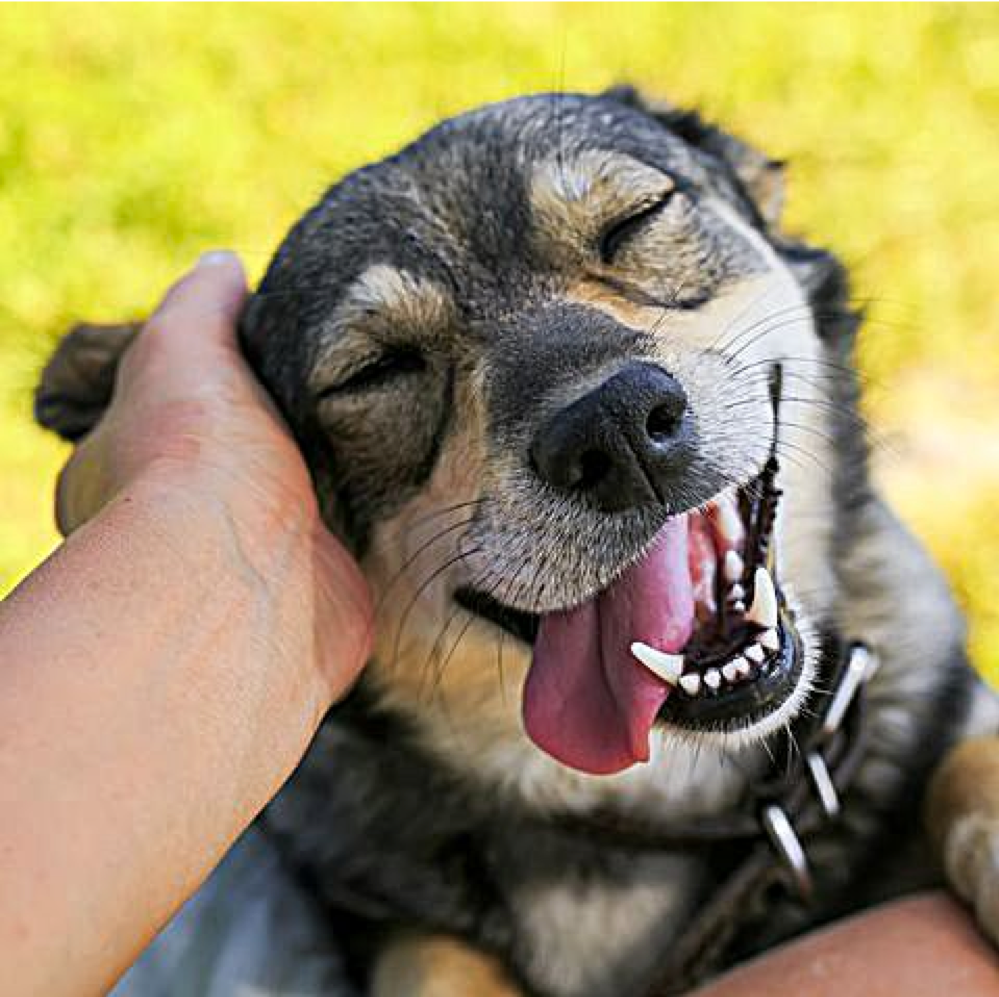
\includegraphics[width=.9\linewidth, right]{pup_sharp.png}  
  \caption{Convolution with the sharpen kernel}
  \label{sb2-3}
\end{subfigure}
\newline
\begin{subfigure}{.3\textwidth}
  \centering
  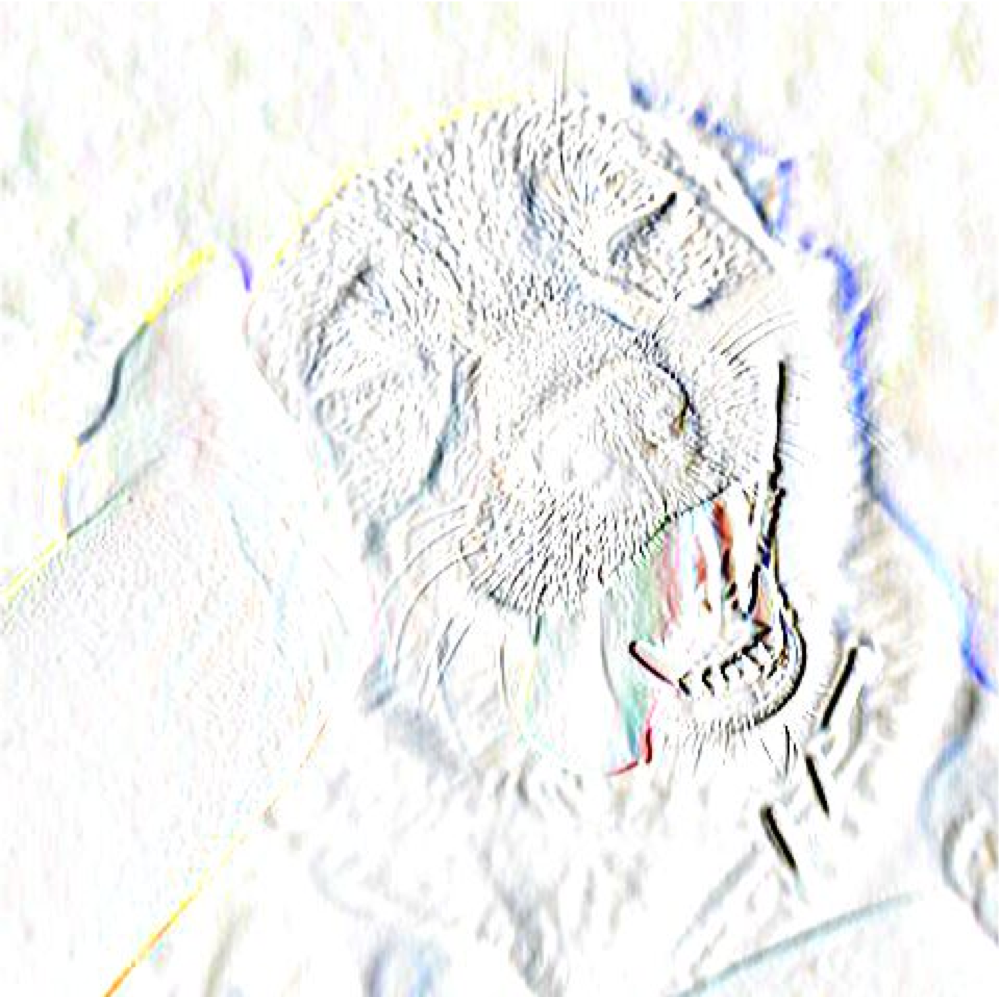
\includegraphics[width=.9\linewidth, left]{pup_sobl1.png}  
  \caption{Convolution with the sobel kernel (positive values) }
  \label{sb2-4}
\end{subfigure}\hspace{5mm}%
\begin{subfigure}{.3\textwidth}
  \centering
  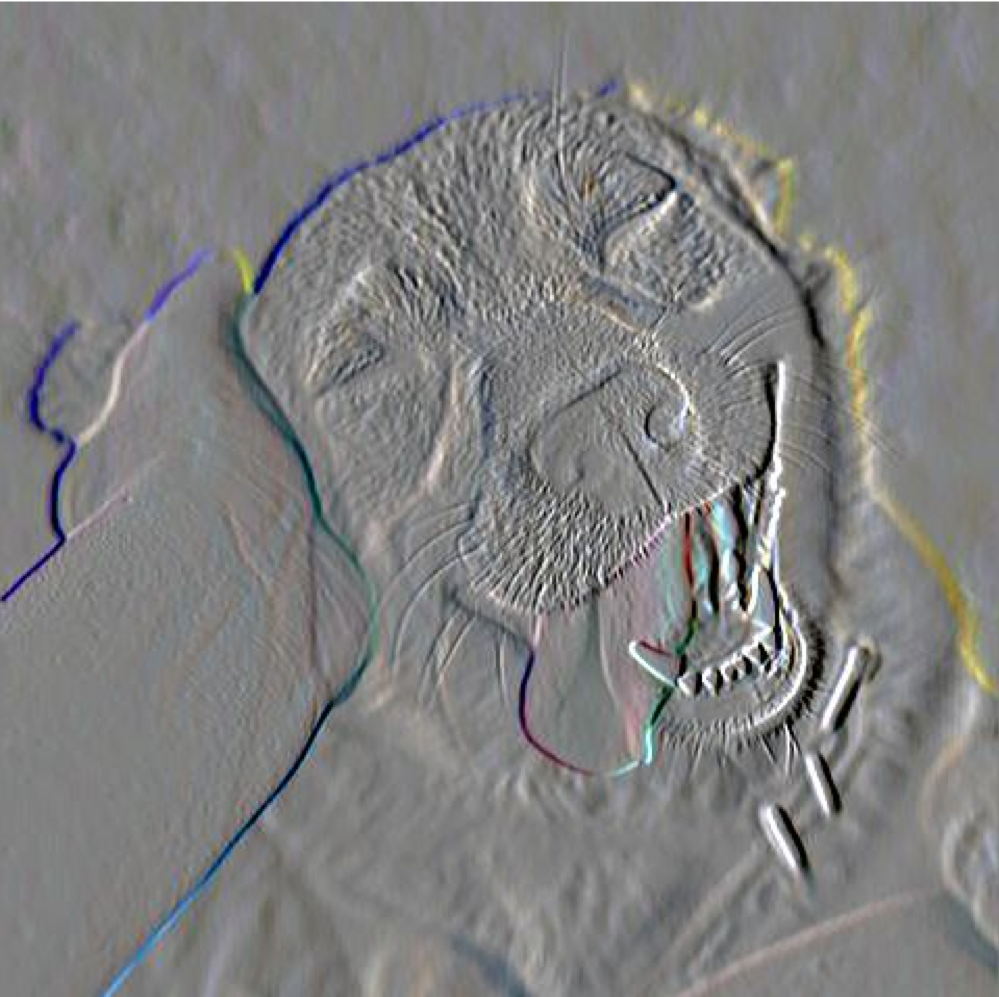
\includegraphics[width=.9\linewidth]{pup_sobl2.png}  
  \caption{Convolution with the sobel kernel (negative values) }
  \label{sb2-5}
\end{subfigure}\hspace{5mm}%
\begin{subfigure}{.3\textwidth}
  \centering
  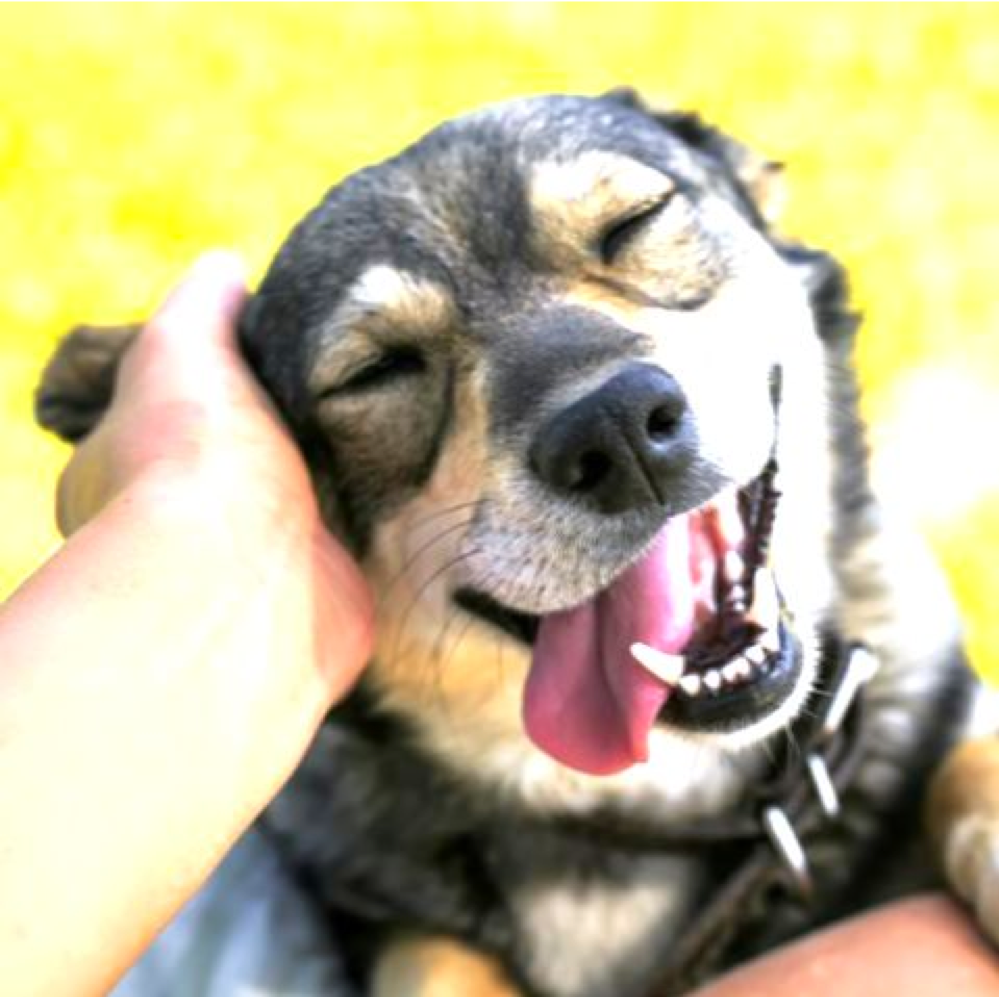
\includegraphics[width=.9\linewidth, right]{pup_blur.png}  
  \caption{Convolution with the blur kernel (hand picked)}
  \label{sb2-6}
\end{subfigure}
	\caption{Use of convolution to change the an image of a dog.}
\label{fig2}
\end{figure}

\section{Section 2: Chi square}
\textit{Identify an application of your interest (preferably of your thesis topic, if you have one) for the chi square test and apply it.} \\

For this application, following the subject of convolution, one of the main topics set for our thesis is the use of Convolutional Neural Networks (CNNs). For this type of Neural Network (NN) we use the same concept that we explained in the convolution section. We take the formula shown in Equation \ref{eq4} and use it to calculate the index and rows of our resulting matrix. \\

 \begin{eqnarray}
\label{eq4}
G[m, n] =  (f*h)[m,n] = \sum_j \sum_k h[j, k]f [m-j, n-k]
\end{eqnarray}

In the case of Convolutional Neural Networks (CNNs) we form a subsequent map of features in each convolution. The kernel used starts with random variables that get fitted in every iteration, depending on the optimizer that we are using. \\

As we can see in Figure \ref{fig1} if we, for example, started with a matrix of $6\times6$ with a kernel of $3\times3$, we will get a feature map of $4\times4$. Since our image shrinks every time we perform a different convolution, we can only perform them a limited number of times before our image disappears completely. That is why there are many architectures of CNN and we experiment to find the best fit for our data.\\

For the experimentation part of this section, first we have to produce data that can be evaluated by the chi squared test. Since the images and and algorithm we are currently working on is a little bit too heavy for the computer we are currently working on, we are using a famous (and digestible for regular computers) data set of images called MNIST Fashion \cite{mnist}, which is widely used as a benchmark in the data science community to validate their algorithms \cite{kaggle}. \\

We run a simple CNN with the help of the library of \texttt{keras}. In Figure \ref{fig2} we show some of the images contained in this data set, and in Table \ref{tab2} we have the results of the model testing, and in Table \ref{tab3} we show the confusion matrix for these classification. \\


\begin{figure}[]
  \centering
  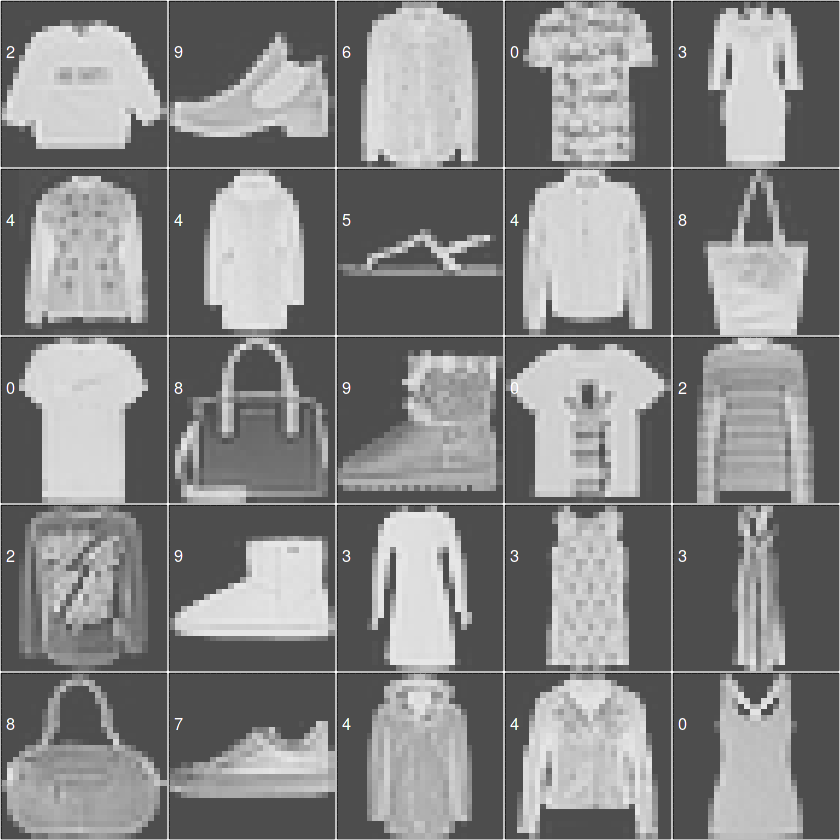
\includegraphics[width=.7\linewidth,]{mnist.png}  
	\caption{Some images form the data set Mnist Fashion.}
\label{fig3}
\end{figure}

\begin{table}[]\caption{Metric results of the CNN model for the classes form the MNIST Fashion data set. }\label{tab2}
\centering
\begin{tabular}{ p{1.5cm} c c c c c c c c c c }
\toprule
Class	&	0	&	1	&	2	&	3	&	4	&	5	&	6	&	7	&	8	&	9	\\
\midrule \\
Sensitivity      	&	88.5\%	&	98.3\%	&	82.4\%	&	90.8\%	&	75.5\%	&	98.3\%	&	67.5\%	&	93.9\%	&	94.4\%	&	93.7\%	\\
Specificity       	&	97.4\%	&	99.7\%	&	97.5\%	&	98.9\%	&	98.4\%	&	99.2\%	&	97.0\%	&	99.3\%	&	99.9\%	&	99.7\%	\\
Pos Pred Value    	&	79.0\%	&	97.0\%	&	78.6\%	&	90.4\%	&	84.1\%	&	93.7\%	&	71.3\%	&	93.8\%	&	98.6\%	&	97.4\%	\\
Neg Pred Value     	&	98.7\%	&	99.8\%	&	98.0\%	&	99.0\%	&	97.3\%	&	99.8\%	&	96.4\%	&	99.3\%	&	99.4\%	&	99.3\%	\\
Prevalence        	&	9.9\%	&	10.1\%	&	10.0\%	&	9.9\%	&	10.1\%	&	10.1\%	&	10.0\%	&	9.9\%	&	9.8\%	&	10.2\%	\\
Detection Rate    	&	8.8\%	&	9.9\%	&	8.3\%	&	9.0\%	&	7.6\%	&	10.0\%	&	6.7\%	&	9.3\%	&	9.3\%	&	9.5\%	\\
Detection Prevalence 	&	11.1\%	&	10.2\%	&	10.5\%	&	10.0\%	&	9.0\%	&	10.6\%	&	9.5\%	&	9.9\%	&	9.4\%	&	9.8\%	\\
Balanced Accuracy   	&	92.9\%	&	99.0\%	&	89.9\%	&	94.9\%	&	86.9\%	&	98.8\%	&	82.3\%	&	96.6\%	&	97.1\%	&	96.7\%	\\
\bottomrule
\end{tabular}
\end{table}

\begin{table}[]\caption{Confusion matrix of prediction results for the CNN model. The principal diagonal represent the correct predictions, and all the other are the wrong predictions.}\label{tab3}
\centering
\begin{tabular}{ c c c c c c c c c c c }
	&	\textbf{0}	&	\textbf{1}	&	\textbf{2}	&	\textbf{3}	&	\textbf{4}	&	\textbf{5}	&	\textbf{6}	&	\textbf{7}	&	\textbf{8}	&	\textbf{9}	\\
\textbf{0}	&	1052	&	1	&	26	&	29	&	1	&	0	&	209	&	0	&	13	&	1	\\
\textbf{1}	&	5	&	1188	&	3	&	18	&	5	&	0	&	5	&	0	&	1	&	0	\\
\textbf{2}	&	15	&	0	&	990	&	2	&	156	&	0	&	90	&	0	&	7	&	0	\\
\textbf{3}	&	18	&	17	&	11	&	1083	&	37	&	0	&	23	&	0	&	9	&	0	\\
\textbf{4}	&	3	&	1	&	67	&	33	&	910	&	0	&	54	&	0	&	14	&	0	\\
\textbf{5}	&	1	&	0	&	0	&	0	&	0	&	1195	&	0	&	50	&	11	&	19	\\
\textbf{6}	&	91	&	1	&	102	&	28	&	97	&	0	&	809	&	0	&	6	&	0	\\
\textbf{7}	&	0	&	0	&	0	&	0	&	0	&	13	&	0	&	1113	&	4	&	57	\\
\textbf{8}	&	4	&	0	&	3	&	0	&	0	&	0	&	8	&	1	&	1115	&	0	\\
\textbf{9}	&	0	&	0	&	0	&	0	&	0	&	8	&	0	&	21	&	1	&	1141	\\
\end{tabular}
\end{table}

To be able to use the confusion matrix represented in Table \ref{tab3} we accommodate the data in a more compact table, as the one shown in Table \ref{tab4}, where we put the right and wrong predictions of each class in two different rows. \\

\begin{table}[]\caption{Table simplifying the data of the confusion matrix made in \texttt{R}.}\label{tab4}
\centering
\begin{tabular}{ p{1.5cm} c c c c c c c c c c }
Class	&	( , 0)	&	( , 1)	&	( , 2)	&	( , 3)	&	( , 4)	&	( , 5)	&	( , 6)	&	( , 7)	&	( , 8)	&	( , 9)	\\
True predictions	&	1052	&	1188	&	990	&	1083	&	910	&	1195	&	809	&	1113	&	1115	&	1141	\\
False predictions	&	277	&	37	&	270	&	115	&	172	&	81	&	325	&	72	&	16	&	30	\\
\end{tabular}
\end{table}

Using the \texttt{chisq.test} \cite{chitest} function in \texttt{R} we get as a result:

\begin{itemize}
\item \textbf{X squared:} 938.25
\item \textbf{df:} 9
\item \textbf{p value:} $< 2.2\times 10^{-16}$
\end{itemize}

So as a conclusion we can say that, in our example, the row and the column variables are statistically significantly associated. And finally, Figure \ref{figextra} shows a bar plot of how the different classes are distributed, being the darker color the correct predictions, and the grey the wrong predictions.  \\

\begin{figure}[]
  \centering
  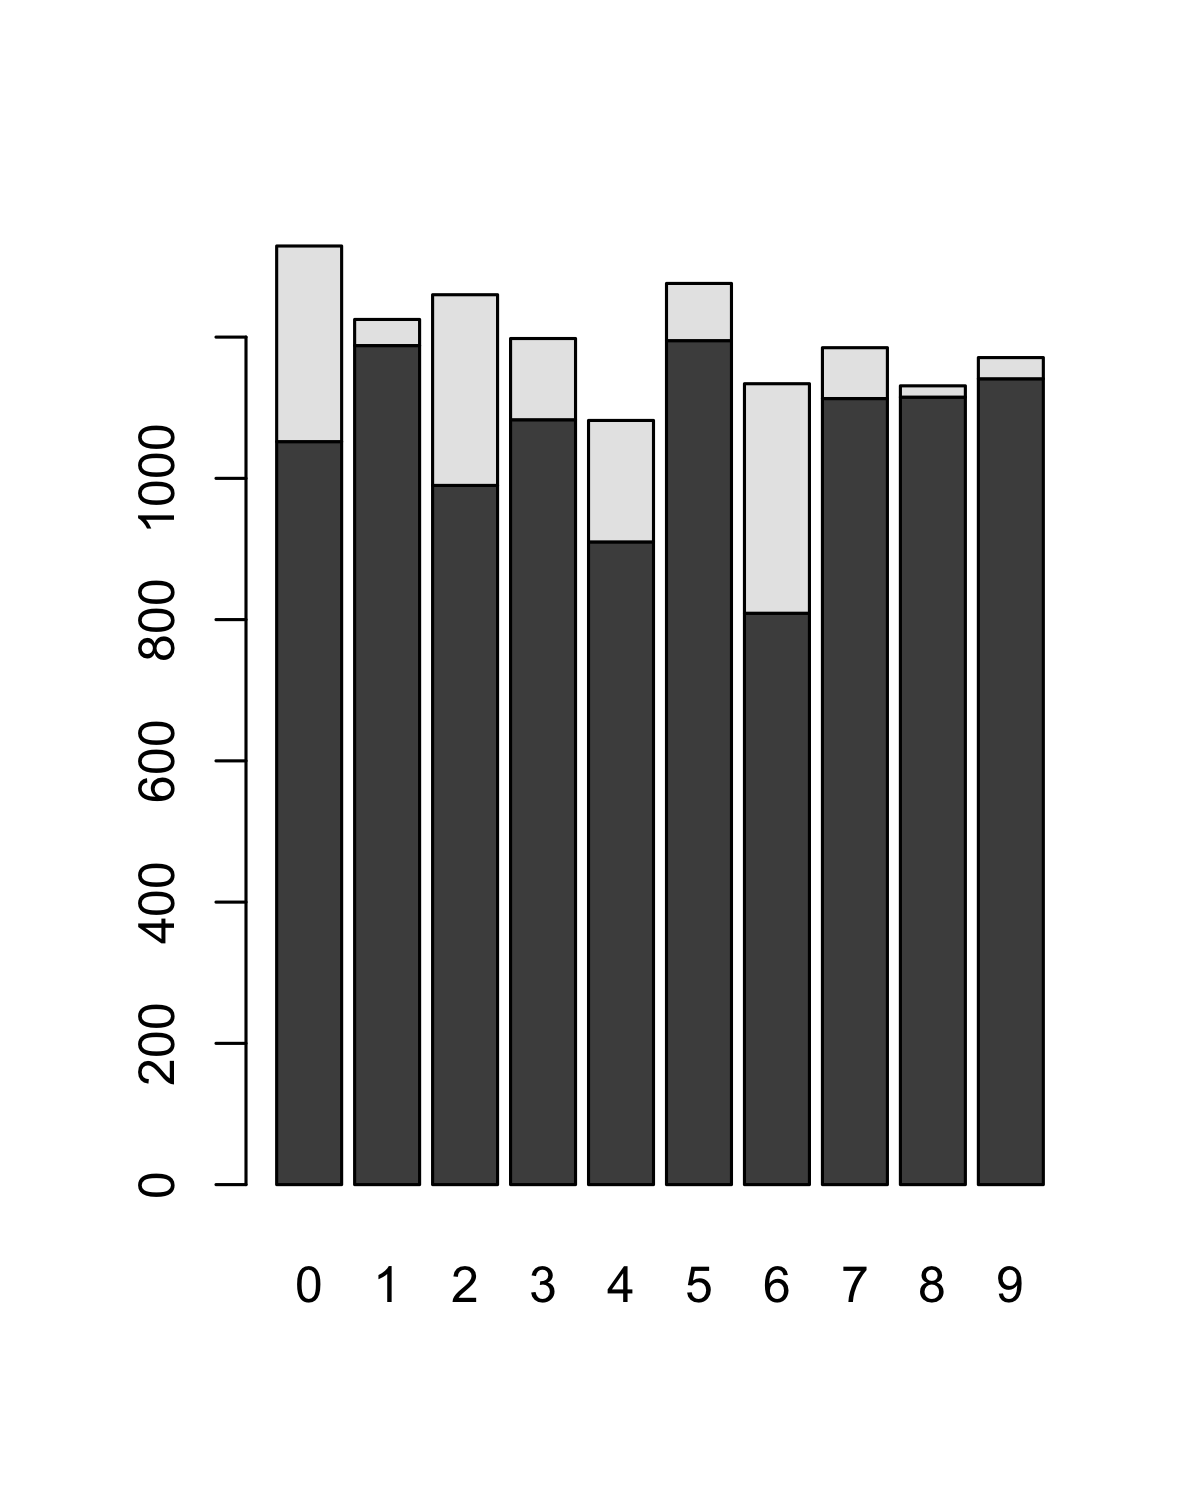
\includegraphics[width=.5\linewidth,]{Ej11_barplot.png}  
	\caption{Barplot of the correct and incorrect predictions of the CNN model on each class.}
\label{figextra}
\end{figure}

\section{Section 3: Covariance}
\textit{Validate the two properties related to the covariance that comes in the class page (preferably, first establish numerically that they are true and then prove them analytically}\\

Both Equation \ref{eq5} and \ref{eq6} come form the example in the class page indicated in the instructions. For Equation \ref{eq6} first we attempt a practical experiment in \texttt{R} using the functions of variance and covariance already in the program, as well as the function of \texttt{sample} to generate the random variables.\\


 \begin{eqnarray}
\label{eq5}
Cov[aX + b, cY + d] =  acCov[X, Y]
\end{eqnarray}

 \begin{eqnarray}
\label{eq6}
Var[X + Y] =  Var[X] - Var[Y] + 2Cov[X, y]
\end{eqnarray}

In Figure \ref{cov} we have the different number of iterations. We went from 10, to 100 to 1000 iterations, in each one we tried the equation with a different number of random variables inside the variance and covariance functions, which can be seen in the \texttt{x} axis of all the plots.\\

The darker color is for all the times the condition of equal was accomplished, and the gray color is when this condition was not met.\\

\begin{figure}[]
\centering
\begin{subfigure}{.76\textwidth}
  \centering
  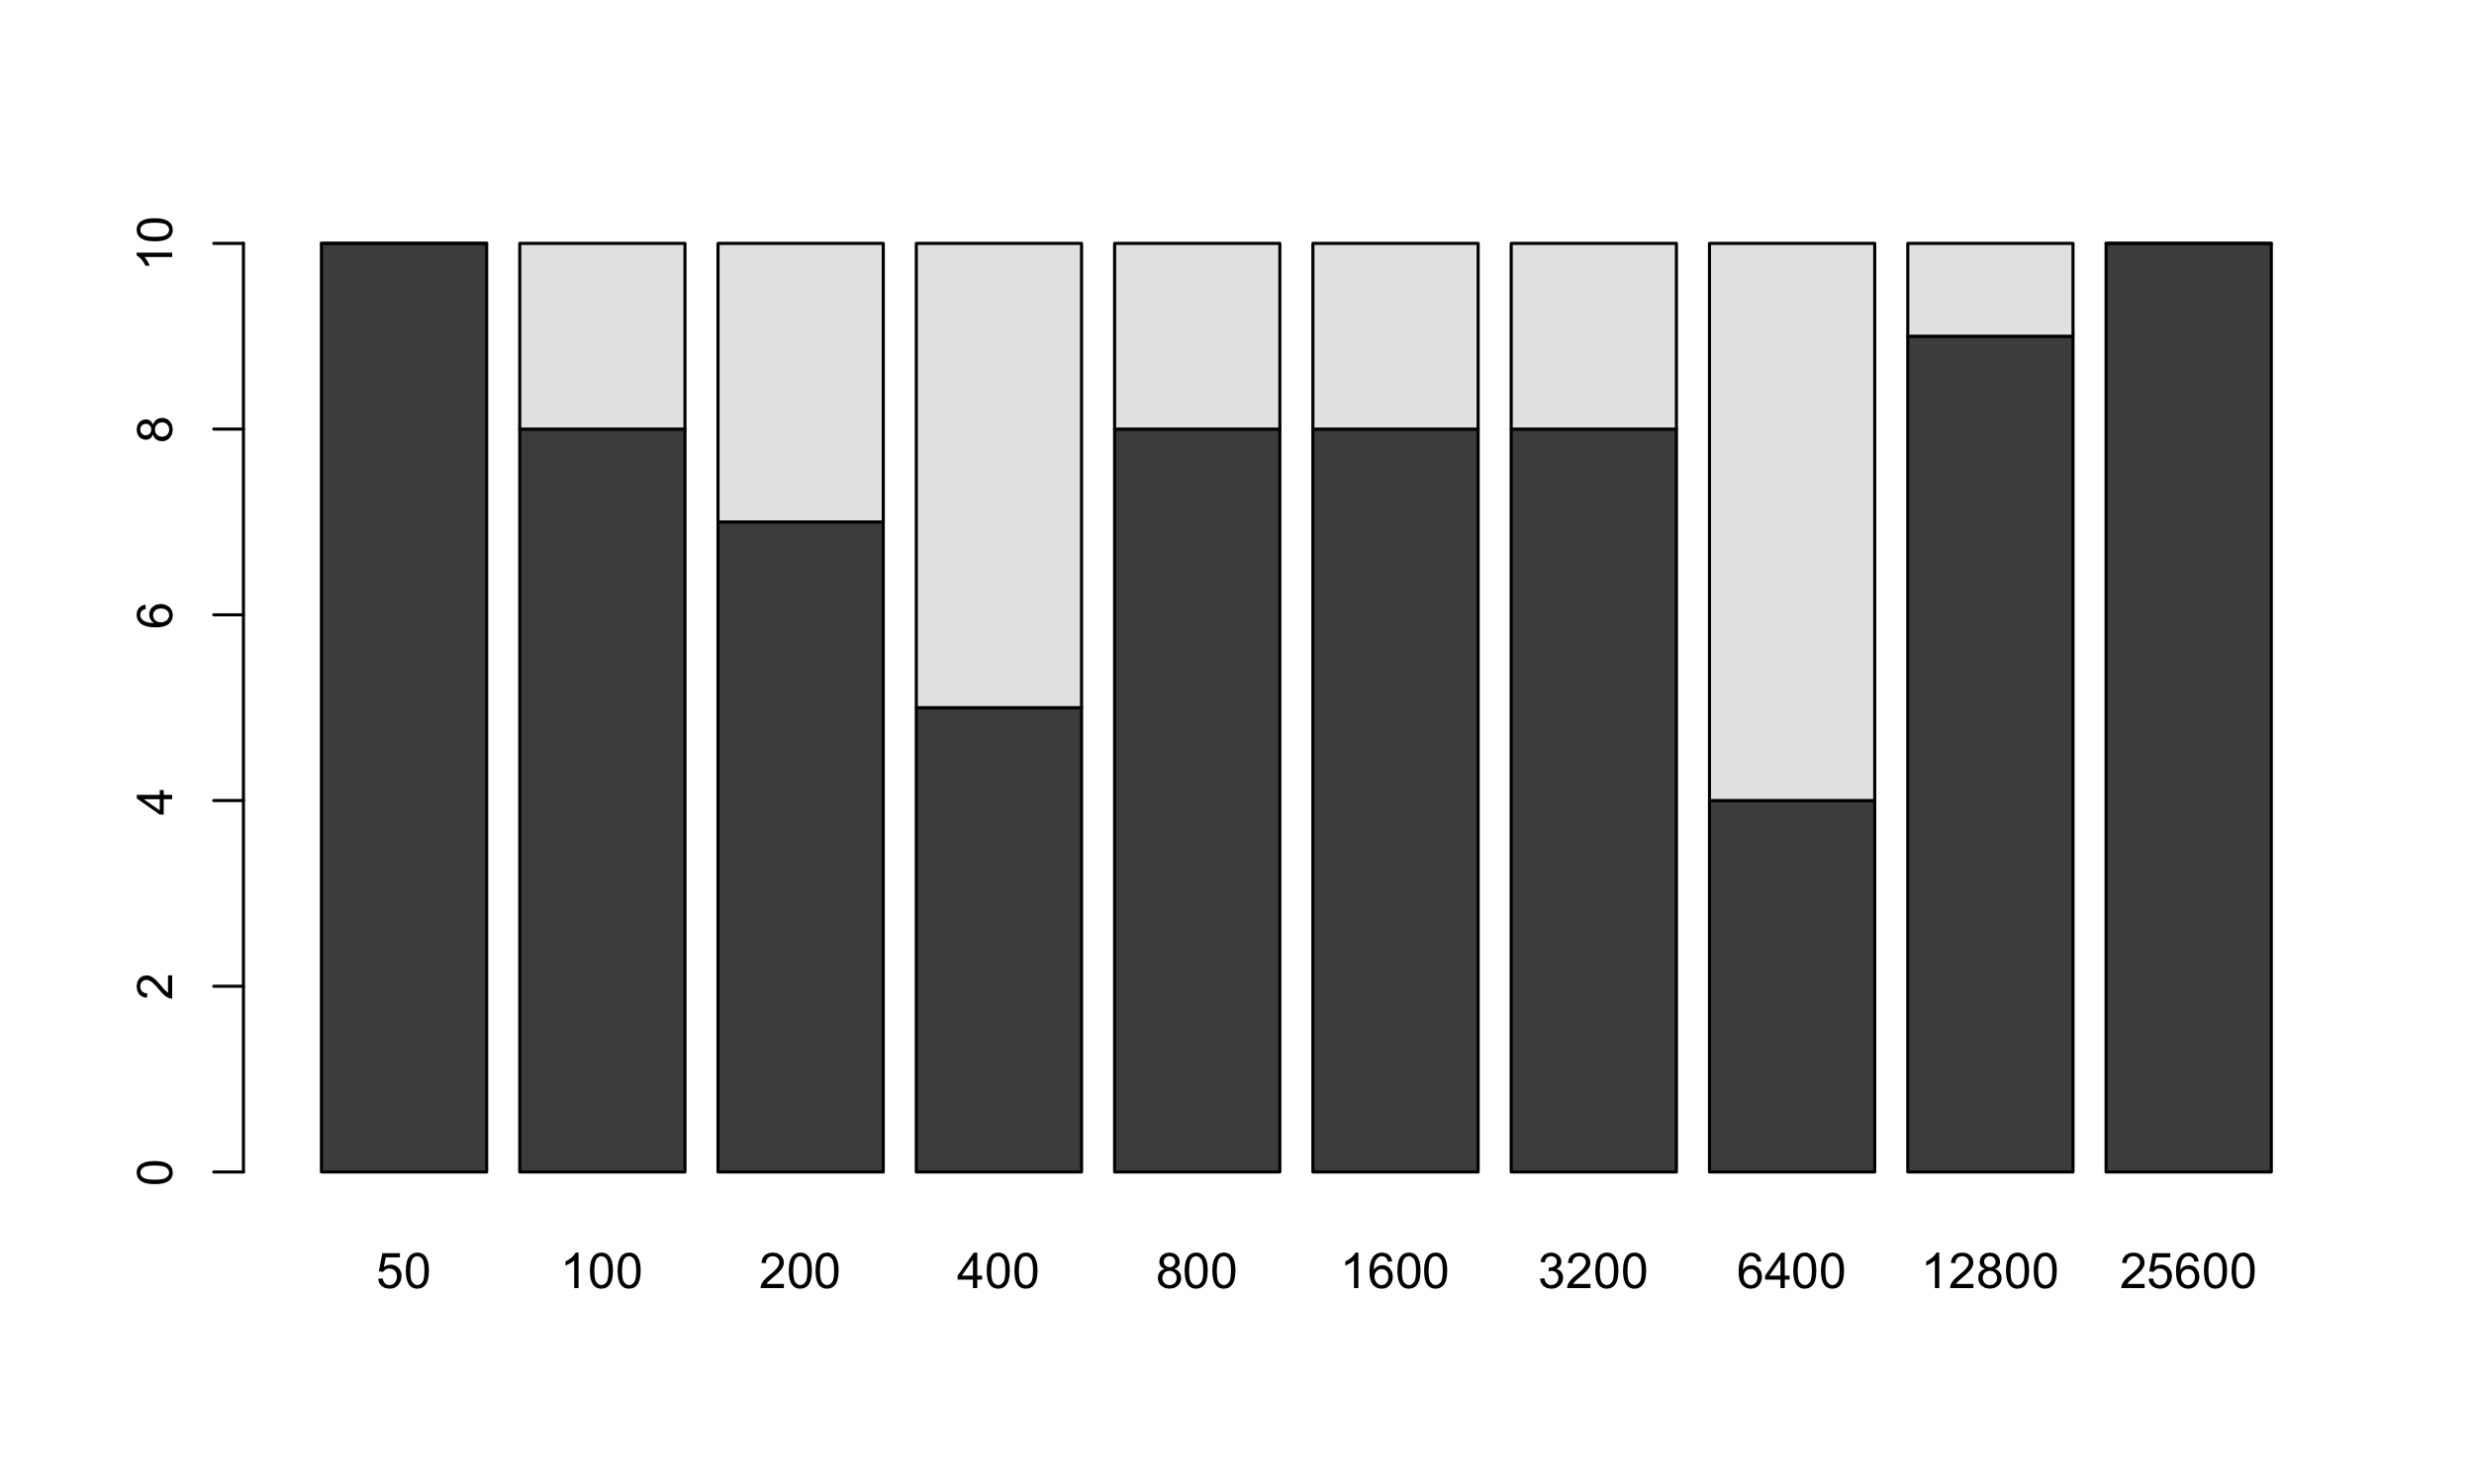
\includegraphics[width=.9\linewidth]{Ej11_barplot4.png}  
  \caption{Barplot from 10 iterations of the equation comparision }
  \label{s1}
\end{subfigure}
\newline
\begin{subfigure}{.76\textwidth}
  \centering
  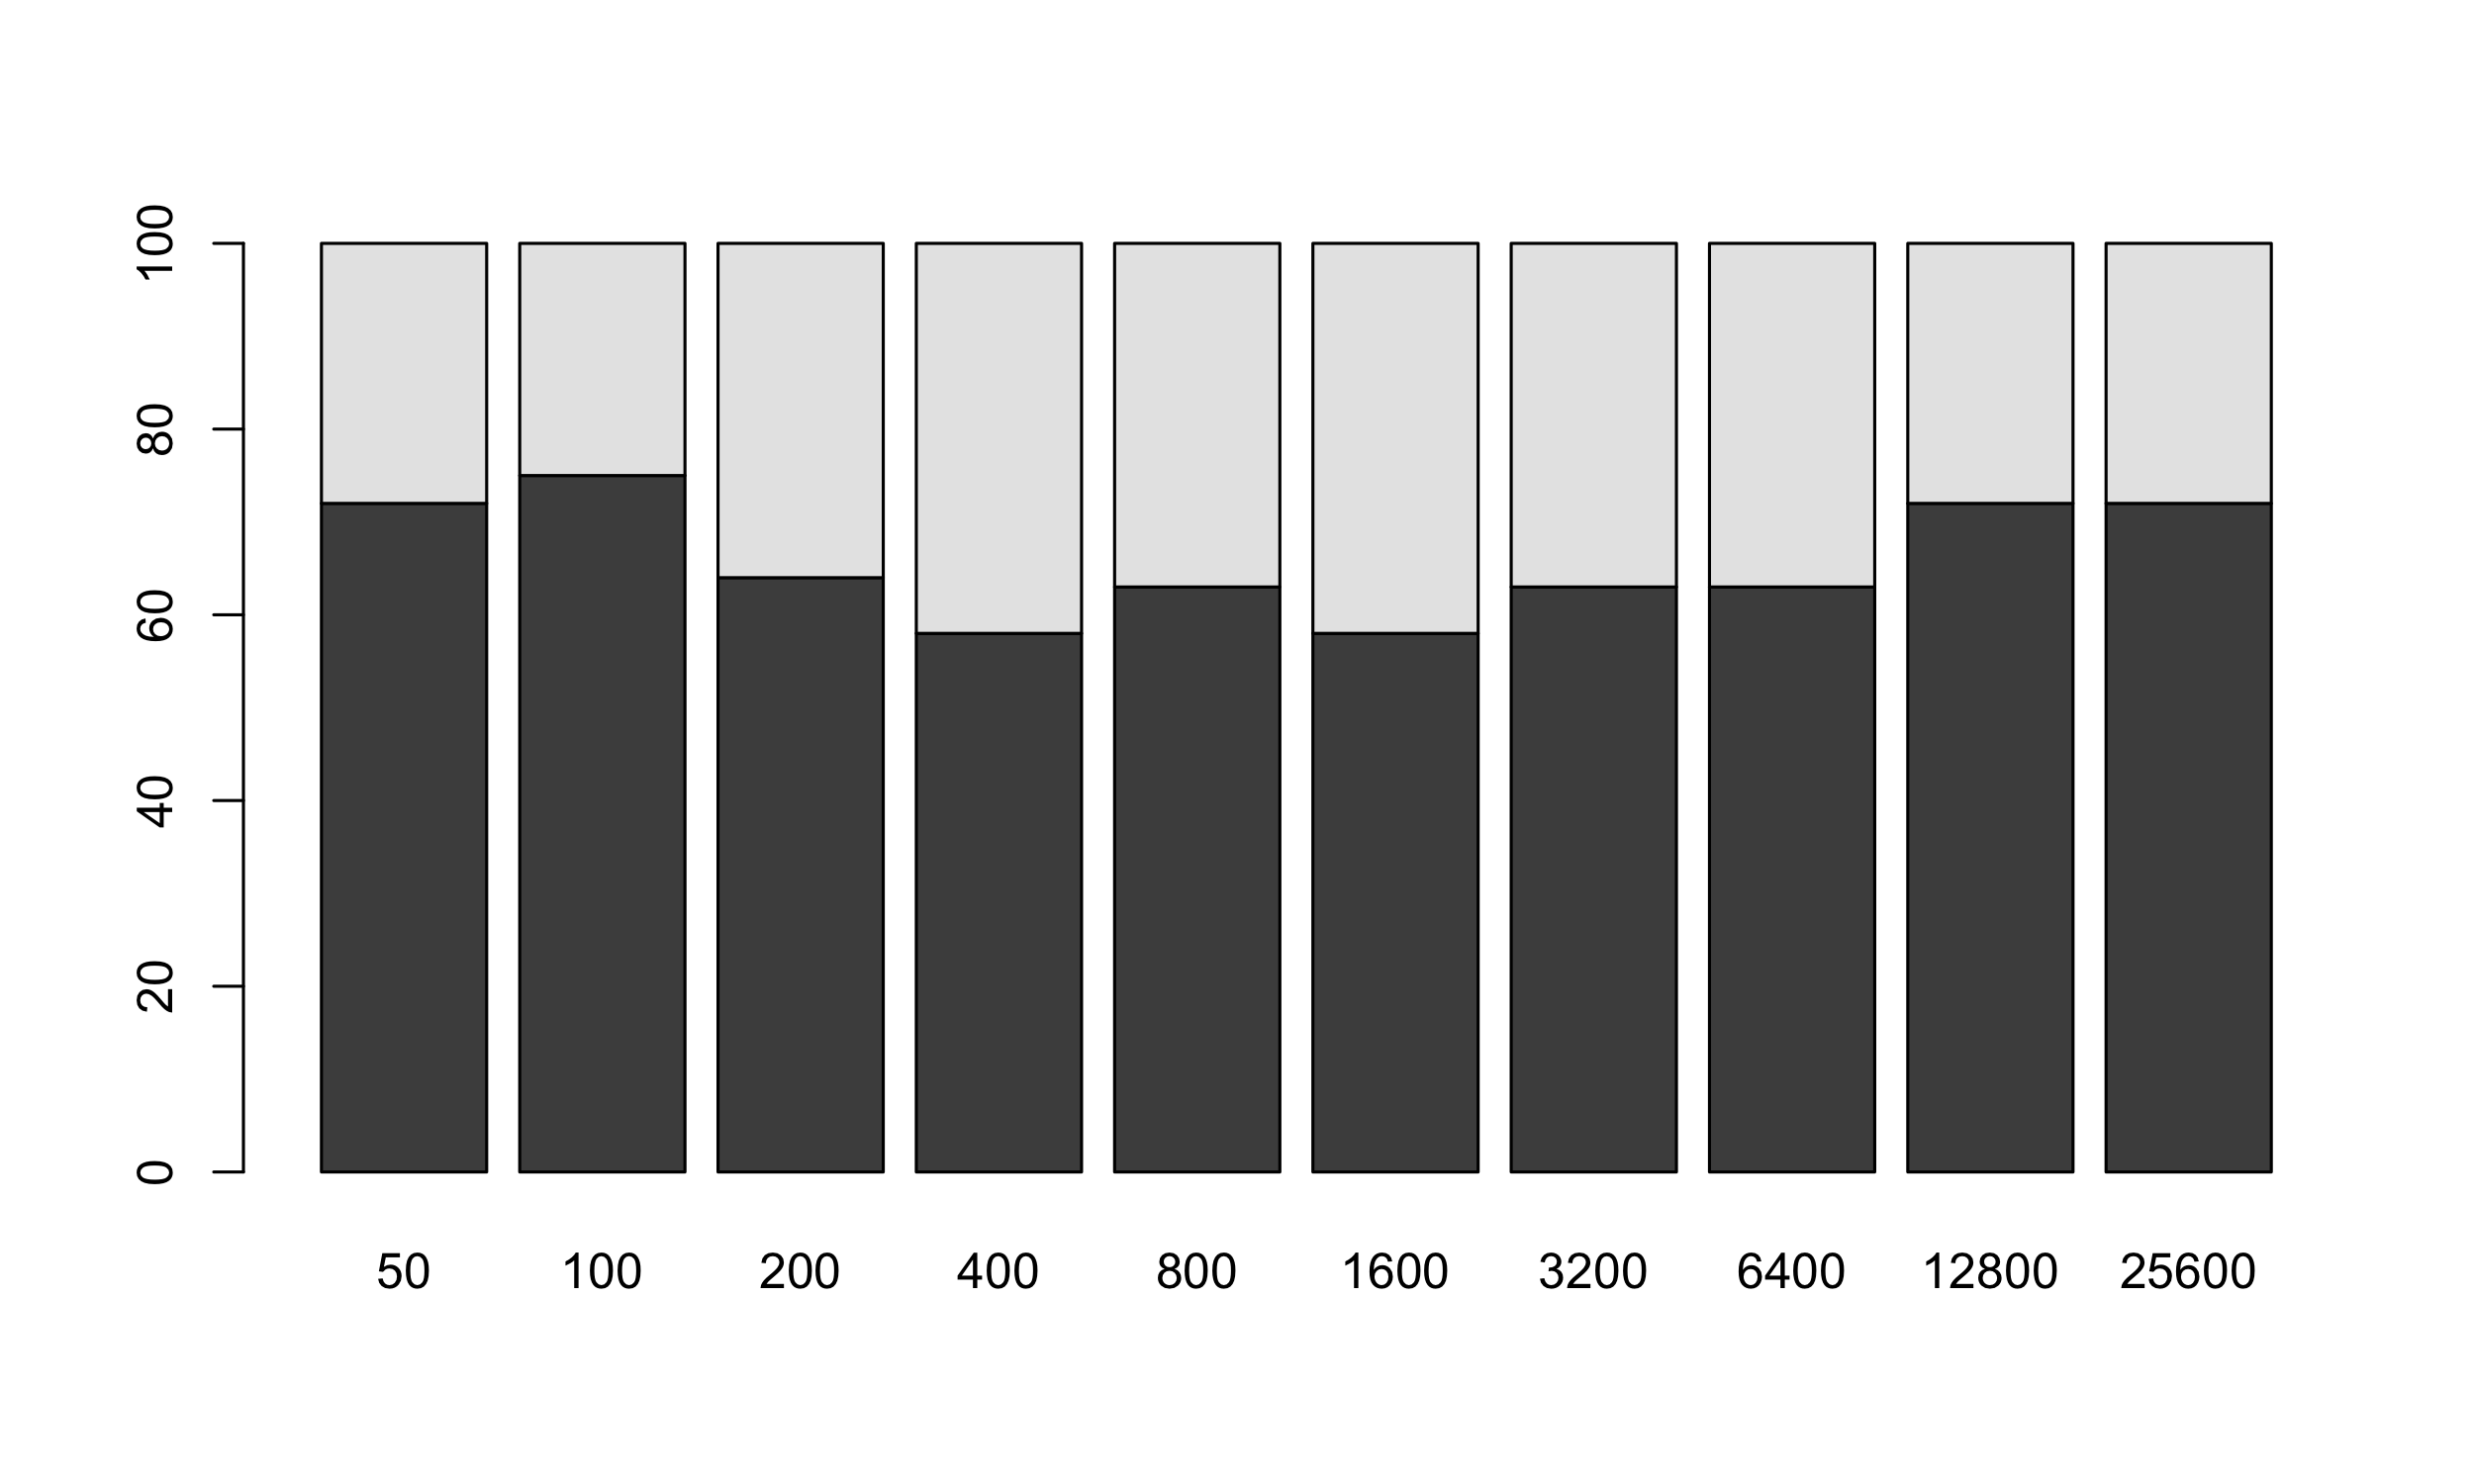
\includegraphics[width=.9\linewidth]{Ej11_barplot3.png}  
  \caption{Barplot from 100 iterations of the equation comparision }
  \label{s2}
\end{subfigure}
\newline
\begin{subfigure}{.76\textwidth}
  \centering
  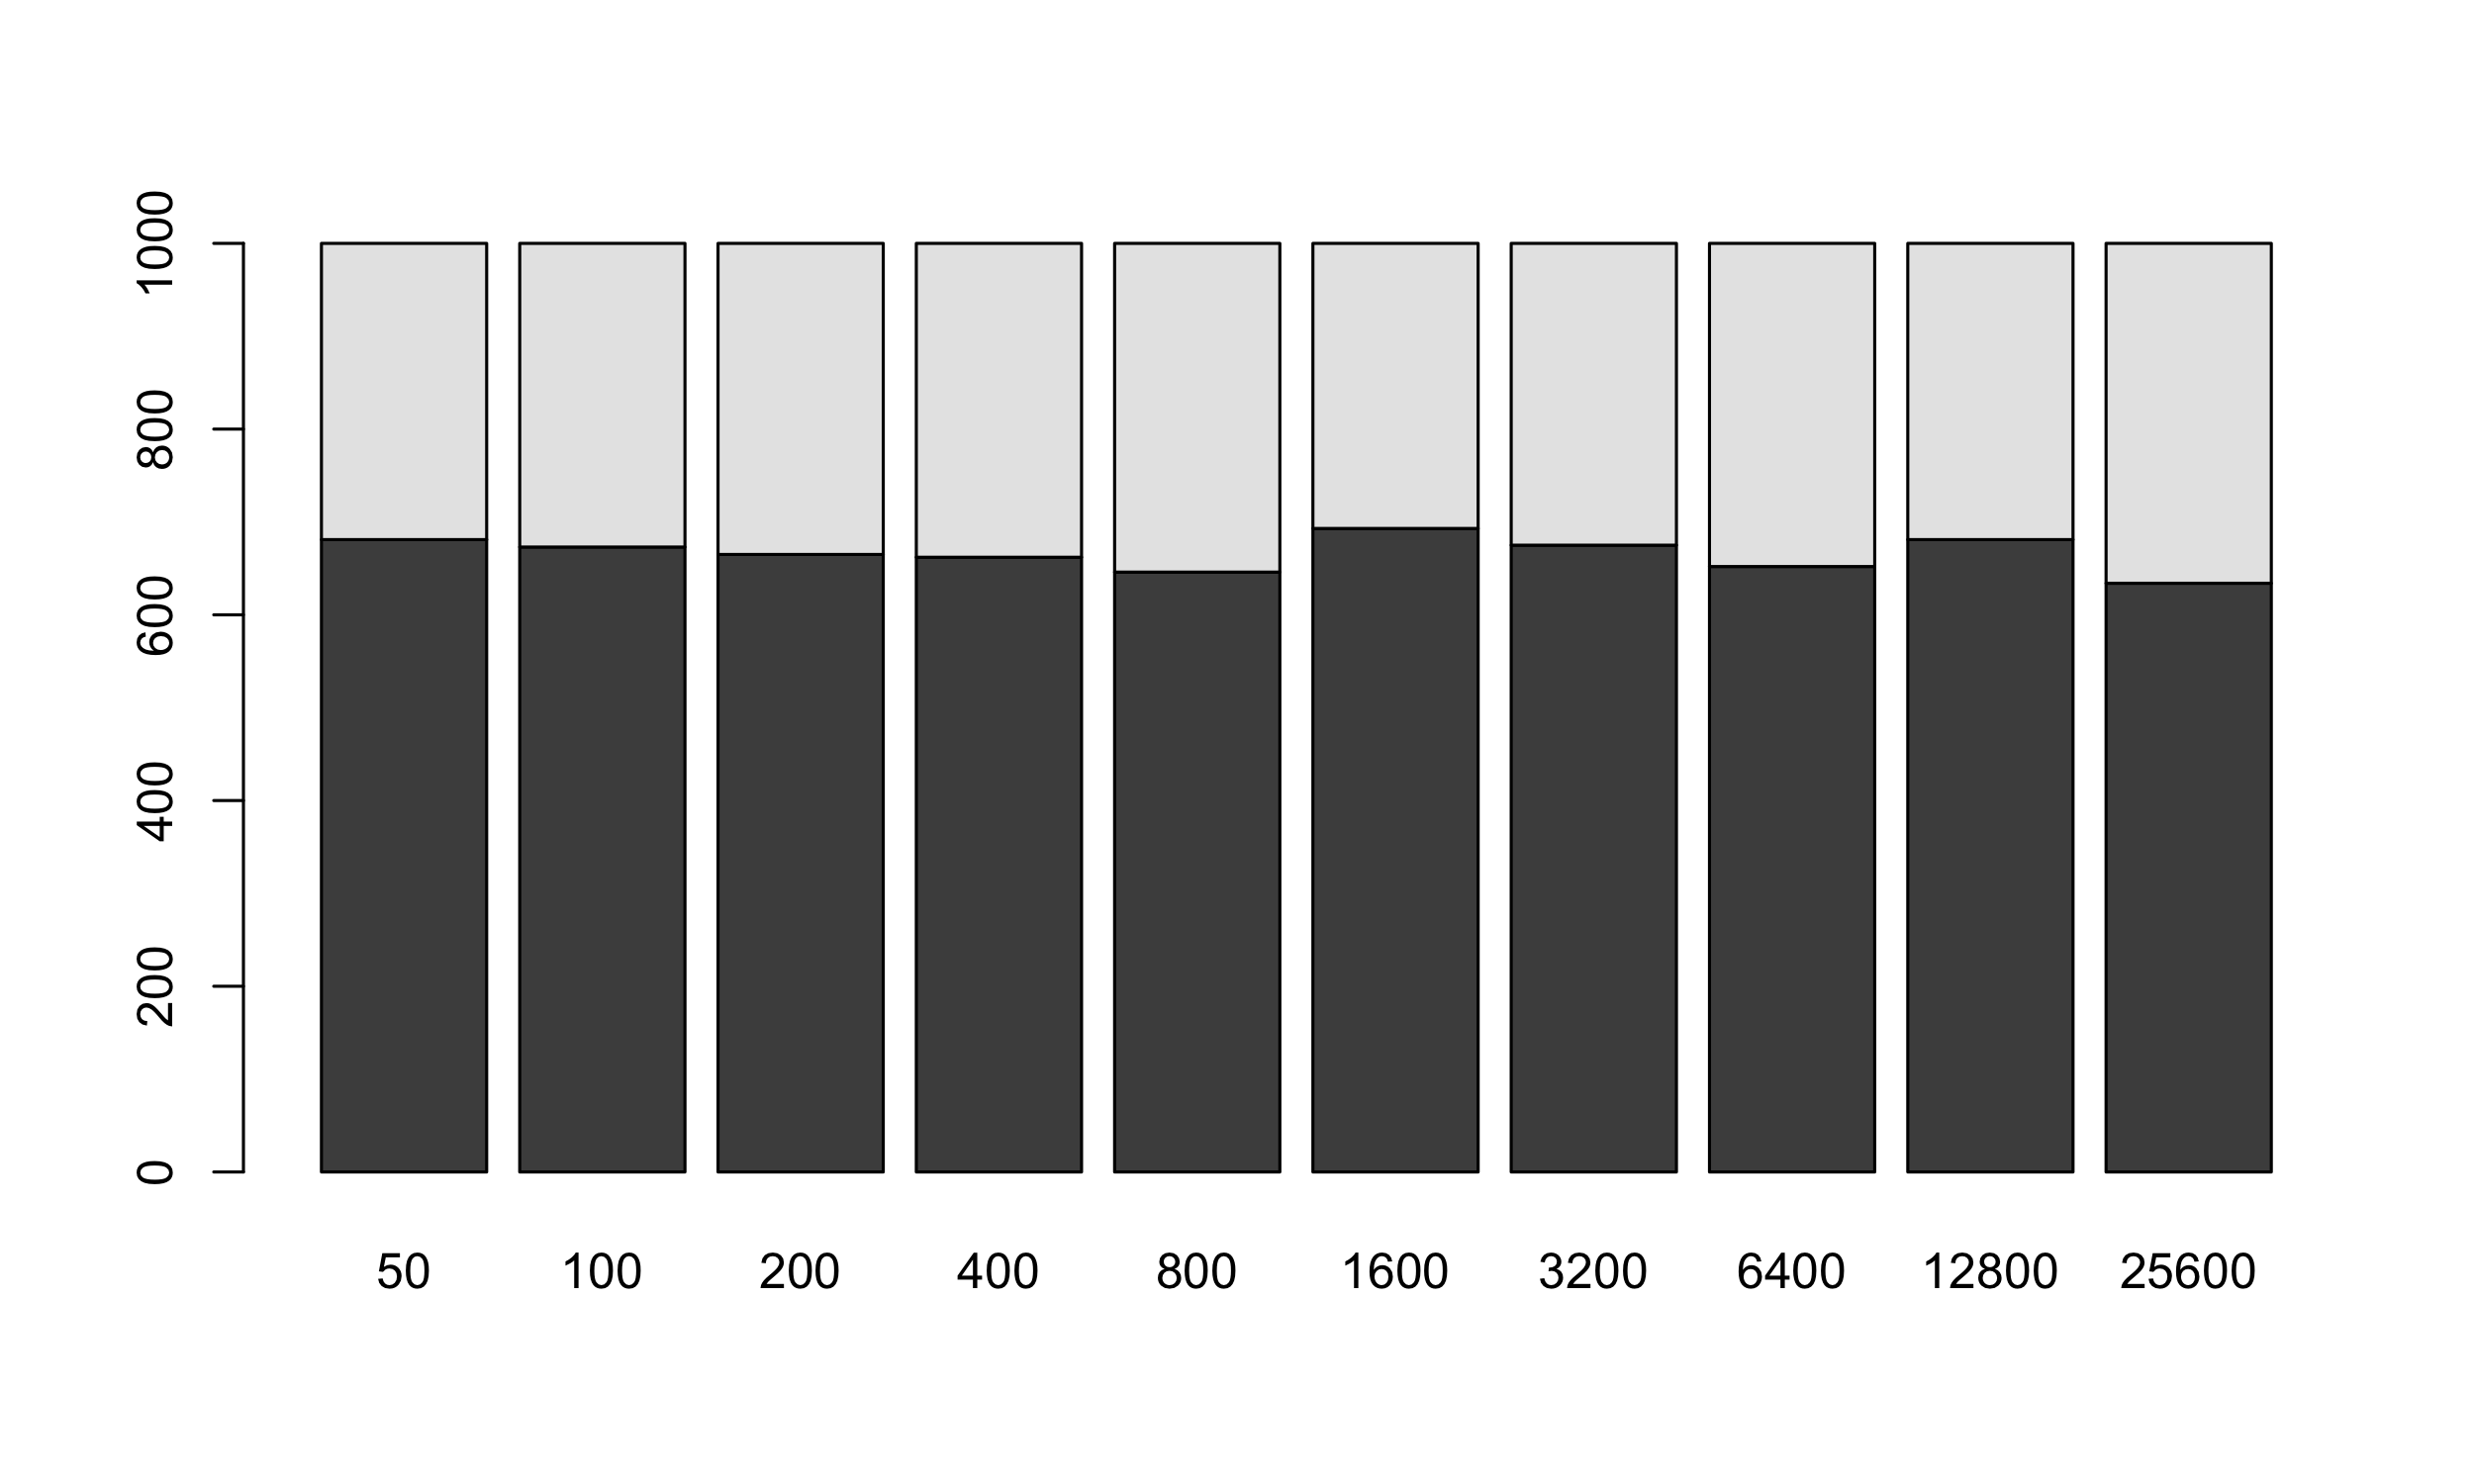
\includegraphics[width=.9\linewidth]{Ej11_barplot2.png}  
  \caption{Barplot from 1000 iterations of the equation comparision }
  \label{s3}
\end{subfigure}
	\caption{Barplots from the different iterations of the experiment of covariance.}
\label{cov}
\end{figure}

The analytic view of the formula can be described by Equation \ref{final} \cite{cova},

\begin{eqnarray}
\label{final}
\begin{split}
Var[X + Y] &\\
=  &\sum_x \sum_y (x+y)^2 P_{XY}(x, y)- (E(X+Y))^2\\
= & \sum_x \sum_y x^2 P_{XY}(x, y) +  \sum_x \sum_y 2xyP_{XY}(x, y) + \\
& \sum_x \sum_y y^2 P_{XY}(x,y) - (E(X))^2 - 2E(X)E(Y)- (E(Y))^2 \\
= &\sum_x x^2 P_{X}(x)-(E(X))2 + \sum_y y^2P_{Y}(y) - (E(Y))^2 +  \\
&\sum_x \sum_y 2xyP_{XY}(x, y) - 2E(X)E(Y)\\
 =& E(X^2) - (E(X))^2 + E(Y^2) - (E(Y))^2 + 2(E(XY)- E(X)E(Y)) \\
 = & Var(X) + Var(Y) + 2Cov(X, Y).
\end{split}
\end{eqnarray}

\section{Conclusion}

As always, I understand better all of this concepts when they come in the form of a practical example. In the reading part leading up to the class I was really confused by the concepts, and the explanations in class where not enough to dispel my doubts. It wasn't until some videos and examples later that I landed on the application of image processing. I thought this convolution and the one seen in class where two different concepts (one for statistics and the other for computer science) but after seeing the application on the example, it became so easy to understand the equations seen class and its uses.\\

In the section of the Chi squared we used the MNIST  dataset because the computer used for the experiments is of average processing capacity, and the images used in the real thesis problem are too big for it to be able to compile the program.\\

\bibliographystyle{plainnat}
\bibliography{tarea11}


 
\end{document}